% !TEX root = ./rosbook_jp.tex
%-------------------------------------------------------------------------------
\chapterimage{chapter_head_2.pdf}

%-------------------------------------------------------------------------------
\chapter{ROS のインストール}

1章で述べたように、ROSは多くのオペレーティングシステムで動作する。しかし、Ubuntu以外のOSは実験的な提供(Experimental)とされており、公式にはサポートされていない。そこで本書では、操作性や導入のしやすさから、UbuntuにインストールされたROSの使用を前提とする。本書で利用するROSの開発環境は、次の通りである。

\begin{itemize}
\item ハードウェア:IntelやAMD製CPUを内蔵したデスクトップおよびノートパソコン
\item オペレーティングシステム:Ubuntu 14.04 LTS または14.04.2 LTS(Trusty Tahr)
\item ROS: Indigo Igloo
\end{itemize}

もしコンピュータにインストールされているUbuntuのバージョンが異なる場合は、対応状況を公式サイト\footnote{\url{http://wiki.ros.org/indigo/Installation/Ubuntu}}で確認する必要がある。オペレーティングシステムがOS XまたはWindowsであれば、それぞれのインストール方法を関連Wiki\footnote{\url{http://wiki.ros.org/indigo/Installation/OSX/Homebrew/Source},\url{http://wiki.ros.org/hydro/Installation/Windows}} で確認されたい。

\begin{figure}[h]
  \centering
  
\includegraphics[width=0.9\columnwidth]{pictures/chapter2/pic_02_01.png}
  \caption{UbuntuのTrustyバージョンとROS Indigoバージョンのロゴ}
\end{figure}

%-------------------------------------------------------------------------------
\section{ROS Indigo のインストール}\index{ROS Indigo のインストール}

%-------------------------------------------------------------------------------
\subsection{ROS Indigo の一般的なインストール方法}\index{ROS Indigo の一般的なインストール方法}

まずROS Indigoのインストール方法について説明する。ただし、以下のインストール手順の説明に登場するソースリストやキーのアドレスは,OSRF財団の運営方針が変わると変更される場合もある。その時は注1のWikiサイトを参照してほしい。

\begin{exercise}[Ubuntuの14.04.2 LTS使用時の問題点]
  2015年2月17日に更新された14.04.2 LTSにROSパッケージをインストールする際、ibgl1-mesa-dri関連の依存関係の問題が起こる。そのため、Ubuntu 14.04.2 LTSをインストールした場合には、ROSをインストールする前に、以下のコマンドを実行して、依存関係ファイルをインストールする必要がある。
  \begin{lstlisting}[language=ROS]
  $ sudo apt-get install libgl1-mesa-dev-lts-utopic
  \end{lstlisting}
\end{exercise}

\subsubsection{NTP(Network Time Protocol) 設定}
ROSの公式な設定項目には含まれてないが、本書では複数のPCでROSを利用することを想定し、NTPの設定を行う。NTPはネットワーク上のPCで時刻同期を行うものである\footnote{\url{http://wiki.ros.org/ROS/NetworkSetup}} 。ROSの基準時間であるROS Timeが各PC間で異なっていると、通信処理に問題が生じるため、以下の2つのコマンドで各PC間のROS Timeを揃える。まず、最初の行のapt-getコマンドでchronyをインストールした後、次の行のntpdateコマンドでntpサーバをntp.ubuntu.com等に指定する。

\begin{lstlisting}[language=ROS]
$ sudo apt-get install chrony
$ sudo ntpdate -q ntp.ubuntu.com
\end{lstlisting}

これにより、各PCの時刻が指定したntpサーバの時刻に同期する。

\subsubsection{ROSリポジトリアドレスの追加}

次のように、ros-latest.listにROSリポジトリアドレスを追加する。

\begin{lstlisting}[language=ROS]
$ sudo sh -c 'echo "deb http://packages.ros.org/ros/ubuntu $(lsb_release -sc) main" > /etc/apt/sources.list.d/ros-latest.list'
\end{lstlisting}

\subsubsection{キーの設定}

ROSリポジトリからパッケージをダウンロードするために公開鍵を追加する。次のように入力する。

\\
\begin{lstlisting}[language=ROS]
$ wget https://raw.githubusercontent.com/ros/rosdistro/master/ros.key -O - | sudo apt-key add -
\end{lstlisting}

\subsubsection{パッケージインデックスの更新}

ソースリストにROSリポジトリアドレスを追加したので、以下のコマンドでパッケージリストをアップデートする。必須ではないが、ROSのインストール前に、インストール済みのUbuntu関連の全てのパッケージを最新のものにしておくとよい。

\\
\begin{lstlisting}[language=ROS]
$ sudo apt-get update && sudo apt-get upgrade
\end{lstlisting}

\subsubsection{ROS Indigo Iglooのインストール}

次のコマンドで、デスクトップ用の基本的なROSパッケージをインストールする。ここには、ROS、rqt、RViz、モデルや位置推定などのロボット関連のライブラリ、シミュレーション、ナビゲーションなどが含まれる。rqtとは、標準的なグラフィカルユーザインタフェースであるQTを利用したROS GUI開発ツールであり、RVizはROS標準の3次元可視化ツールである。これらは5章でより詳細に取り上げる。

\begin{lstlisting}[language=ROS]
$ sudo apt-get install ros-indigo-desktop-full
\end{lstlisting}

上記のコマンドを実行すれば基本的なrqtはインストールされるが、本書ではrqt関連のすべてのパッケージをインストールすることを推奨する。次のコマンドでrqt関連のすべてのパッケージがインストールでき、これにより様々なrqtプラグインが利用できる。

\begin{lstlisting}[language=ROS]
$ sudo apt-get install ros-indigo-rqt*
\end{lstlisting}

\begin{exercise}[ROSパッケージのバイナリのインストール]
  他のROSパッケージをインストールしたい場合には、次のようにapt-cacheのコマンドを利用して、ros-indigoで始まるパッケージを検索する。現在、以下のコマンドを実行すると、約1,600個のパッケージを確認することができる。

  \begin{lstlisting}[language=ROS]
  $ sudo apt-cache search ros-indigo*
  \end{lstlisting}

  個々のパッケージをインストールしたい場合は、次のコマンドでインストールする。

  \begin{lstlisting}[language=ROS]
  $ sudo apt-get install ros-indigo-%*[パッケージ名]*)
  \end{lstlisting}

  apt-cacheやapt-getコマンド以外にも、GUIツールであるsynaptic package managerを利用することもできる。
\end{exercise}

\begin{exercise}[APT(Advanced Packaging Tool)]
  apt-get、apt-key、apt-cache等で出てくるaptはAdvanced Packaging Toolの略語で、Ubuntuを含めDebian系列のLinuxでよく使用されるパッケージ管理コマンドである。

  http://en.wikipedia.org/wiki/Advanced\_Packaging\_Tool
\end{exercise}

\begin{exercise}[以前のバージョンのROSの削除と他のROSバージョンの併用]
  sudo apt-get purge ros-[以前のバージョン]-*コマンドで、以前のバージョンに関連したすべてのファイルが削除できる。もし、既存のバージョンと併用したい場合には、.bashrcに追加したROS設定ファイルを取得するコマンドの中で

  \begin{lstlisting}[language=ROS]
source /opt/ros/indigo/setup.bash
  \end{lstlisting}

  太文字を利用したいバージョンに変更すれば、複数のバージョンのROSを切り替えて利用できる。

 ※Ubuntuのバージョンが利用したいROSバージョンをサポートしている時のみ可能。1章参照のこと。
\end{exercise}

\subsubsection{rosdepの初期化}
ROSをインストールした後は、一度rosdepを初期化する必要がある。rosdepとは、rosの主要コンポーネントの使用時、もしくはコンパイル時に、依存関係にあるパッケージのインストールを容易にするツールである。

\begin{lstlisting}[language=ROS]
$ sudo rosdep init
$ rosdep update
\end{lstlisting}

\subsubsection{rosinstallのインストール}
続いて、ROSの様々なパッケージを容易にインストールするためのプログラムであるrosinstallをインストールしよう。必須ではないが、使用頻度が高く便利なツールであることから、本書ではrosintallのインストールを推奨する。

\begin{lstlisting}[language=ROS]
$ sudo apt-get install python-rosinstall
\end{lstlisting}

\subsubsection{環境設定ファイルのロード}

環境設定ファイルをロードする。 ファイルにはROS\_ROOT、ROS\_PACKAGE\_PATHなどの環境変数が定義されている。

\begin{lstlisting}[language=ROS]
$ source /opt/ros/indigo/setup.bash
\end{lstlisting}

\subsubsection{作業フォルダの作成と初期化}

ROSはcatkinというROS専用ビルドシステムを使用している。これを使用するには、次のコマンドでcatkin作業フォルダを作成し、作業フォルダ内の初期化を行う必要がある。この設定はROSインストールの後に一度だけ行えばよい。

\begin{lstlisting}[language=ROS]
$ mkdir -p ~/catkin_ws/src
$ cd ~/catkin_ws/src
$ catkin_init_workspace
\end{lstlisting}

catkin作業フォルダを作成した後、試しに作業フォルダ内のプログラムをビルドしてみよう。この時点では、catkin作業フォルダにはsrcフォルダとその中のCMakeLists.txtというファイルしか入っていないが、次のようにcatkin\_makeコマンドを使用してビルドする。

\begin{lstlisting}[language=ROS]
$ cd ~/catkin_ws/
$ catkin_make
\end{lstlisting}

問題なくビルドが完了したら、次のようにlsコマンドでフォルダの中身を確認しよう。

\begin{lstlisting}[language=ROS]
$ ls
build devel src
\end{lstlisting}

既にあるsrcフォルダのほかに、buildフォルダ、develフォルダが新たに作成されているのが分かる。catkinビルドシステムのビルドに関連するファイルはbuildフォルダに、実行に関連するファイルはdevelフォルダに保存される。
最後に、catkinビルドシステムに関連する環境ファイルを呼び出そう。

\begin{lstlisting}[language=ROS]
$ source ~/catkin_ws/devel/setup.bash
\end{lstlisting}

\subsubsection{テスト}
これで、ROSのインストールがすべて終了した。正しくインストールされたかを確認するため、一度すべてのターミナルウィンドウを閉じて、新しいターミナルウィンドウを開き、次のコマンドを入力してroscoreを実行してみよう。

\begin{lstlisting}[language=ROS]
$ roscore
\end{lstlisting}

次のようにエラーがなく実行された場合、インストールは正しく完了している。

\begin{lstlisting}[language=ROS]
$ roscore
... logging to /home/rt/.ros/log/f4b17da6-ecda-11e4-a7bf-d43d7e970cb0/roslaunch-rt-18869.log
Checking log directory for disk usage. This may take a while.
Press Ctrl-C to interrupt
Done checking log file disk usage. Usage is <1GB.

started roslaunch server http://192.168.4.100:47915/
ros_comm version 1.11.10


SUMMARY
========

PARAMETERS
 * /rosdistro: indigo
 * /rosversion: 1.11.10

NODES

auto-starting new master
process[master]: started with pid [18881]
ROS_MASTER_URI=http://192.168.4.100:11311/

setting /run_id to f4b17da6-ecda-11e4-a7bf-d43d7e970cb0
process[rosout-1]: started with pid [18894]
started core service [/rosout]
\end{lstlisting}

ROSを終了するには、<Ctrl>+<c>を押す。

%-------------------------------------------------------------------------------
\subsection{ROS Indigo の簡単インストール}\index{ROS Indigo の簡単インストール}

2.1.1項ではROS標準のインストール方法について説明したが、Ubuntuのバージョンが13.10か14.04であれば、前述したROSのインストールを自動的に実行するスクリプトを準備した。これを利用すれば、容易にROSをインストールできる。
※ただし、インストールできるROSのバージョンはIndigoのみである。

\begin{lstlisting}[language=ROS]
$ wget https://raw.githubusercontent.com/irvs/rosbook/master/ros_indigo_install.sh
$ sh ros_indigo_install.sh
\end{lstlisting}

%-------------------------------------------------------------------------------
\section{ROS の開発環境の構築}\index{ROS の開発環境の構築}

%-------------------------------------------------------------------------------
\subsection{ROS の環境設定}\index{ROS の環境設定}

ここまででROSがインストールできたので、次にROSが実行できるようにUbuntuの環境設定を行う。以下に示す手順で環境設定を行わない場合、ROSのインストールの途中で行った環境設定ファイルの読み込みは、新しいターミナルウィンドウを開く度に、次のコマンドにより行わなければならない。

\begin{lstlisting}[language=ROS]
$ source /opt/ros/indigo/setup.bash
$ source ~/catkin_ws/devel/setup.bash
\end{lstlisting}

これは非常に煩わしいので、新しいターミナルウィンドウを開くたびに、定められた環境設定ファイルを読み込むように設定する。またそれに加えて、ROSネットワークの設定や、頻繁に使用するコマンドの短縮形を登録しておくとよい。以下で手順を説明する。
まず、geditなどの文書編集プログラムを使用して、ユーザーのホームディレクトリ(/home/[ユーザー名]/)にある「.bashrc」ファイルを変更しよう。次のコマンドで「.bashrc」ファイルを開く。文章編集プログラムとして、gedit以外にsublime text、vim、emacs、nanoなどを使用しても構わない。

\begin{lstlisting}[language=ROS]
$ gedit ~/.bashrc
\end{lstlisting}

「.bashrc」ファイルを読み込むと、既に多くの環境設定がされている。設定済みの部分には触れずに、「.bashrc」ファイルの一番下までスクロールし、次の内容を追加する。6行目のxxx.xxx.xxx.xxxには、使用しているPCのIPアドレスを入れる。IPアドレスは「ifconfig」コマンドで確認できる。

~/.bashrc ファイルの追加部分
\begin{lstlisting}[language=bash]
1: # Set ROS Indigo
2: source /opt/ros/indigo/setup.bash
3: source ~/catkin_ws/devel/setup.bash
4:
5: # Set ROS Network
6: export ROS_HOSTNAME=xxx.xxx.xxx.xxx
7: export ROS_MASTER_URI=http://${ROS_HOSTNAME}:11311
8:
9: # Set ROS alias command
10: alias cw='cd ~/catkin_ws'
11: alias cs='cd ~/catkin_ws/src'
12: alias cm='cd ~/catkin_ws && catkin_make'
\end{lstlisting}

「.bashrc」ファイルを保存した後、修正された「.bashrc」ファイルの設定を反映させるために、現在開いているターミナルウィンドウで次のコマンドを入力する。

\begin{lstlisting}[language=bash]
$ source ~/.bashrc
\end{lstlisting}

%-------------------------------------------------------------------------------
\subsubsection{ROSの環境設定ファイルの読み込み}

「.bashrc」ファイルで、「#」で始まる行はコメント行であり、設定に影響を与えない。追加部分の2行目の「source /opt/ros/indigo/setup.bash」と3行目の「source ~/catkin\_ws/devel/setup.bash」を設定することで、ターミナル起動時にROSの環境設定ファイルが読み込まれる。

%-------------------------------------------------------------------------------
\subsubsection{ROSネットワーク設定}

「.bashrc」の追加部分の6~7行目はROSネットワークに関する記述であり、ROS\_MAS TER\_URIとROS\_HOSTNAMEを設定する意味をもつ。ROSはTCP/IPネットワークを利用した通信を行うため、この設定は極めて重要である。現段階では、どちらも使用しているPCのIPアドレスを入力すれば良い。今後、ROSネットワーク全体を統括するPC(マスターPC、roscoreを起動するPC)が一台だけ別にあり、複数台のロボットでそれぞれマスターPCとは異なるPC(ホストPC)を使用する場合、これらを分けて入力すると、異なるPC間で通信が可能になる。次に、マスターPC、ホストPCともに現在使用しているPCであり、このPCのIPアドレスが192.168.4.100である場合の設定例を示す。

\begin{lstlisting}[language=bash]
# Set ROS Network
export ROS_HOSTNAME=192.168.4.100
export ROS_MASTER_URI=http://${ROS_HOSTNAME}:11311
\end{lstlisting}

\begin{exercise}[ifconfig]
  Linuxで使用しているPCのIPアドレスを調べるには、ifconfigコマンドを利用する。以下の例のようにターミナルウィンドウでifconfigを実行してみよう。有線ならeth、無線であればwlanの項目で、inet addr以降の部分が使用しているPCのIPアドレスである。次の例では、有線接続時のIPアドレスは192.168.4.100である。
  \begin{lstlisting}[language=ROS, backgroundcolor=\color{ocre!10}, numbers=none]
  $ ifconfig
  eth0 Link encap:Ethernet HWaddr xx:xx:xx:xx:xx:xx
  inet addr:192.168.4.100 Bcast:192.168.4.255 Mask:255.255.255.0
  inet6 addr: fexx::d6xx:7exx:f1xx:xx2/64 Scope:Link

  lo  Link encap:Local Loopback
  inet addr:127.0.0.1 Mask:255.0.0.0 inet6 addr: ::1/128 Scope:Host

  wlan1 Link encap:Ethernet HWaddr xx:xx:xx:xx:xx:xx
  inet addr:192.168.4.200 Bcast:192.168.4.255 Mask:255.255.255.0
  inet6 addr: fexx::23xx:dfxx:fexx:5exx/64 Scope:Link
  \end{lstlisting}
\end{exercise}

%-------------------------------------------------------------------------------
\subsubsection{短縮コマンドの設定}

前掲の「.bashrc」の追加部分の10~12行目からは、ROSの開発作業で頻繁に使用するコマンドの短縮形を設定している。

\begin{itemize}[leftmargin=*]
\item cw:あらかじめ設定しておいたcatkin作業フォルダである~/catkin\_wsに移動
\item cs:catkin作業フォルダの中のソースファイルのフォルダである~/catkin\_ws/srcに移動
\item cm:catkin作業フォルダの~/catkin\_wsに移動した後、catkin\_makeコマンドでROSパッケージをビルド
\end{itemize}

\begin{exercise}[ROSの環境設定を確認する方法]
  次のように「export|grep ROS」コマンドを利用してROSの環境設定を確認できる。

  \begin{lstlisting}[language=bash]
  $ export | grep ROS
  declare .x ROS_DISTRO="indigo"
  declare .x ROS_ETC_DIR="/opt/ros/indigo/etc/ros"
  declare .x ROS_HOSTNAME="192.168.4.100"
  declare .x ROS_MASTER_URI="http://192.168.4.100:11311"
  declare .x ROS_PACKAGE_PATH="/home/xxx/catkin_ws/src:/opt/ros/indigo/share:/opt/ros/indigo/ stacks"
  declare .x ROS_ROOT="/opt/ros/indigo/share/ros"
  declare .x ROS_TEST_RESULTS_DIR="/home/xxx/catkin_ws/build/test_results"
  \end{lstlisting}
\end{exercise}


%-------------------------------------------------------------------------------
\subsection{ROSの動作テスト}\index{ROSの動作テスト}

ROSをインストールした後、正常に動作するかを確認するために、ROSが提供する簡単なノード(☞用語集P.XXX)の実行方法について説明する。使用するのはturtlesimというパッケージで、これは、ROSのシンボルである亀が画面に表示され、キーボード操作によって移動するプログラムである。

%-------------------------------------------------------------------------------
\subsubsection{roscoreの実行}

新しいターミナルウィンドウを開いて、次のコマンドを実行する。これにより、すべてのROSシステムを管理するroscoreが起動される。

\begin{lstlisting}[language=ROS]
$ roscore
\end{lstlisting}

\begin{figure}[h]
  \centering
  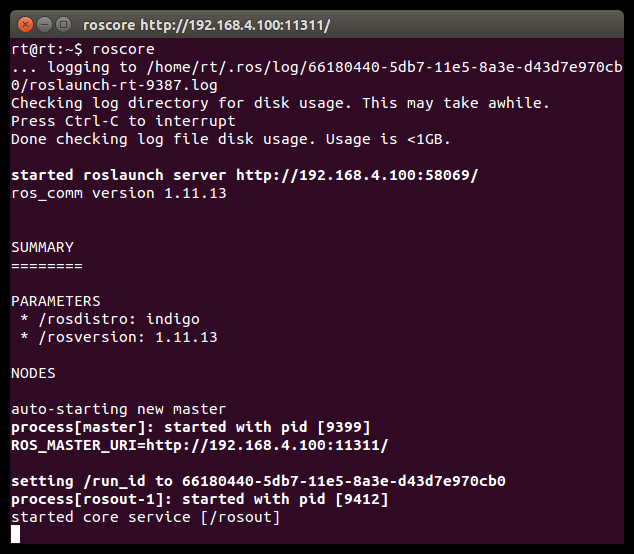
\includegraphics[width=0.9\columnwidth]{pictures/chapter2/pic_02_02.png}
  \caption{roscoreが起動された画面}
\end{figure}

%-------------------------------------------------------------------------------
\subsubsection{turtlesimパッケージのturtlesim\_nodeの実行}

新しいターミナルウィンドウを開いて、次のコマンドを実行する。

\begin{lstlisting}[language=ROS]
$ rosrun turtlesim turtlesim_node
[INFO] [1430205691.820701916]: Starting turtlesim with node name /turtlesim
[INFO] [1430205691.827666004]: Spawning turtle [turtle1] at x=[5.544445], y=[5.544445], theta=[0.000000]
\end{lstlisting}

これを実行すると、メッセージがいくつか表示され、turtlesimパッケージのturtlesim \_nodeが実行される。そして図2-6のように、青い背景のウィンドウに亀が表示される。亀の形状はランダムに変化するため、図2-6と形状が異なる場合がある。

\begin{figure}[h]
  \centering
  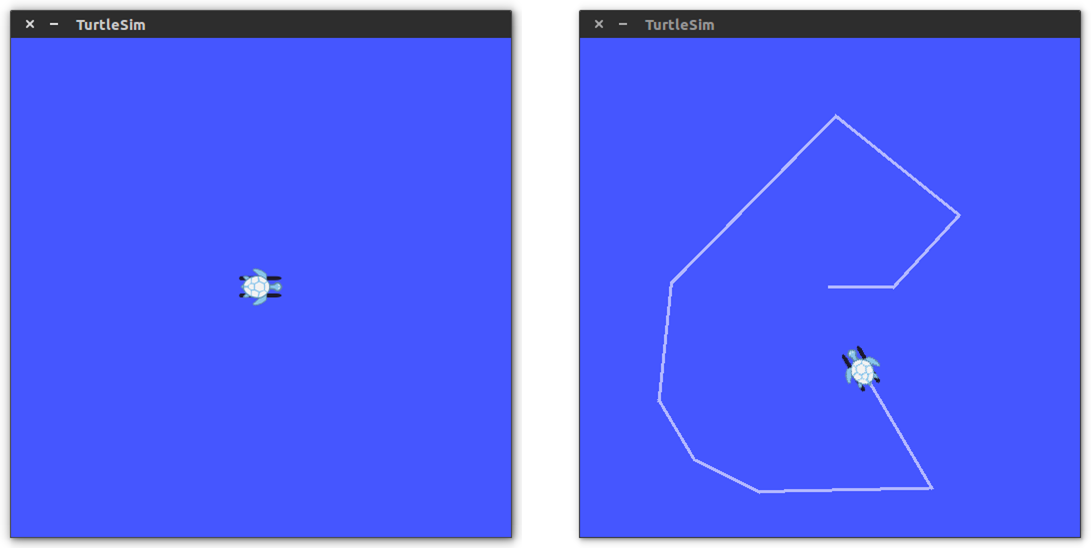
\includegraphics[width=0.9\columnwidth]{pictures/chapter2/pic_02_03.png}
  \caption{turtlesim\_nodeのウィンドウ: (a) 起動時 (b) 亀を移動させた様子}
\end{figure}

turtlesimパッケージのturtle\_teleop\_key実行
別の新しいターミナルウィンドウを開いて、次のコマンドを実行する。

\begin{lstlisting}[language=ROS]
$ rosrun turtlesim turtle_teleop_key
Reading from keyboard
...........................
Use arrow keys to move the turtle.
\end{lstlisting}

これによりメッセージがいくつか表示され、turtlesimパッケージのturtle\_teleop\_keyが実行される。turtle\_teleop\_keyを実行したターミナルウィンドウで、キーボードの方向キー(←、→、↑、↓)を押すと、図2-6(b)のように亀が方向キーに応じて動くことが確認できる。これは2つのノード間の通信を利用した簡単な遠隔制御シミュレーションであるが、実際のロボットもこのような方法で遠隔制御することができる。後半の章で、ロボットの遠隔制御について取り上げる。

%-------------------------------------------------------------------------------
\subsubsection{実行中のノードの確認}

rqt\_graphノードは、現在実行中のノードの情報を見ることができるGUI形式のノードである。このrqt\_graphノードを用いて、実行中のノードを確認してみよう。まず、新しいターミナルウィンドウを開いて、次のコマンドを実行する。

\begin{lstlisting}[language=ROS]
$ rosrun rqt_graph rqt_graph
\end{lstlisting}

これにより、rqt\_graphパッケージのrqt\_graphノードが実行され、図2-7のようなグラフが確認できる。
楕円はノード(/teleop\_turtle、/turtlesim)を意味し、四角はトピック(/turtle1/cmd\_vel)を意味する。teleop\_turtle、turtlesim はそれぞれ、turtle\_teleop\_keyノード、turtlesim\_nodeノードの実行名である。外側の3つの四角(teleop\_turtle、turtle1、turtlesim)は異なるグループであることを示している。図2-7を詳細に見てみよう。/teleop\_turtleノードから矢印が引かれて/turtlesimにつながっている。これは、両方のノードが実行中で、両方のノードの間にはトピックメッセージ(/turtle1/cmd\_vel)通信が行われていることを表す。つまり、turtle\_teleop\_keyノードから、ユーザーのキーボードコマンドがロボットのシミュレーターであるturtlesim\_nodeノードに渡されている。ノード間のトピックメッセージ通信については、後半の章で取り上げる。
以上でROS動作テストは完了である。ここまでスムーズに進行した場合、問題無くROSがインストールされている。

\begin{figure}[h]
  \centering
  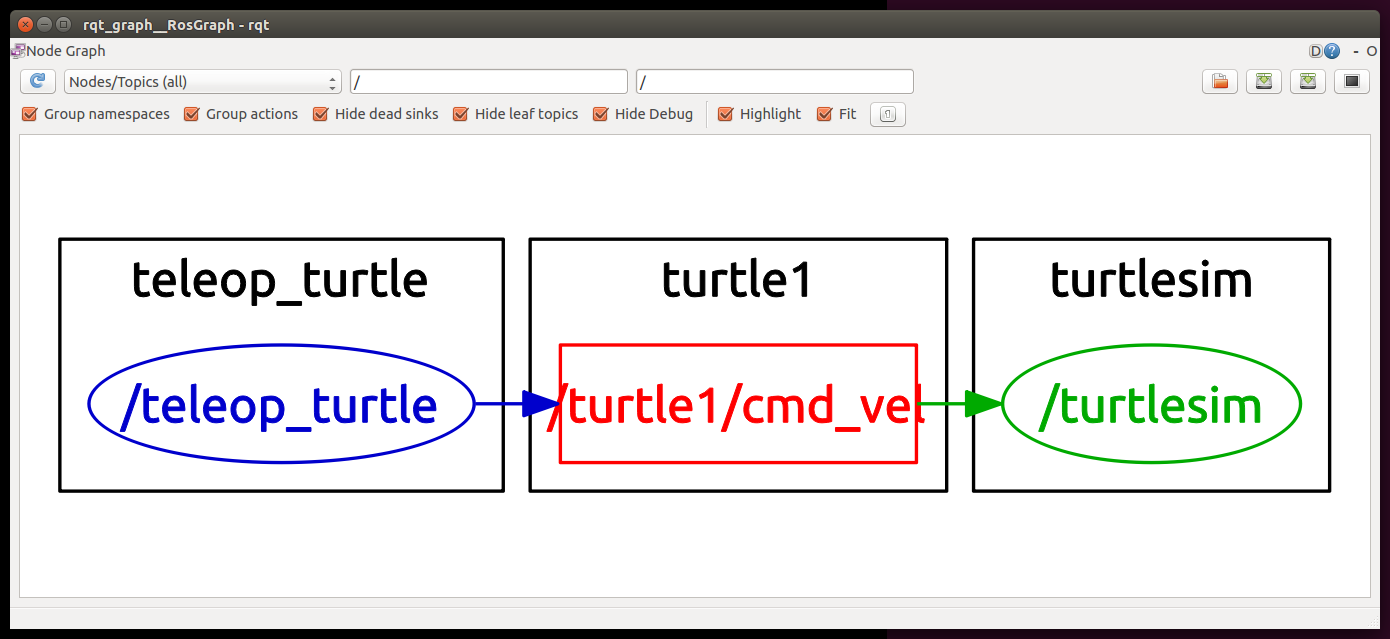
\includegraphics[width=0.9\columnwidth]{pictures/chapter2/pic_02_04.png}
  \caption{rqt\_graphノード}
\end{figure}

%-------------------------------------------------------------------------------
\subsubsection{ノードの終了}
実行されたroscoreとノードを終了する際は、ターミナルウィンドウで<Ctrl>+<c>を押す。

%-------------------------------------------------------------------------------
